\documentclass[conference]{IEEEtran}
% Korean translation support (xelatex + kotex)
\usepackage{kotex}
\usepackage{fontspec}
\setmainfont{NanumMyeongjo}[AutoFakeSlant=0.167]
\setsansfont{NanumGothic}[AutoFakeSlant=0.167,AutoFakeBold=2.0]
\setmainhangulfont{NanumMyeongjo}[AutoFakeSlant=0.167]
\setsanshangulfont{NanumGothic}[AutoFakeSlant=0.167,AutoFakeBold=2.0]
\setmonohangulfont{NanumGothicCoding}[AutoFakeSlant=0.167]
\setmonofont{NanumGothicCoding}[AutoFakeSlant=0.167]
\linespread{1.20}\selectfont
\renewcommand{\figurename}{그림}
\renewcommand{\tablename}{표}
\setlength{\parindent}{1.2em}
\usepackage{graphicx}
\usepackage{tabularx}
\usepackage{booktabs}
\usepackage{array}
\usepackage{titlesec}
\usepackage{fancyvrb}
\usepackage{hyperref}
\hypersetup{colorlinks=true,linkcolor=blue,urlcolor=blue,citecolor=blue}
\newcolumntype{Y}{>{\raggedright\arraybackslash}X}
\titleformat{\section}{\normalfont\normalsize\bfseries\sffamily}{\thesection.}{0.6em}{}
\titleformat{\subsection}{\normalfont\normalsize\bfseries\sffamily}{\thesubsection}{0.6em}{}
\titlespacing*{\section}{0pt}{1.5ex plus .5ex}{0.8ex}
\titlespacing*{\subsection}{0pt}{1.2ex plus .4ex}{0.5ex}
\DefineVerbatimEnvironment{code}{Verbatim}{fontsize=\scriptsize,frame=single,framesep=3pt,xleftmargin=2pt}

\title{Loop Engineering: 에이전트를 프롬프트하는 시스템을 설계하기 위한 Anthropic 플레이북}
\author{공개 PDF에서 재구성한 한국어 번역본\\\textit{원본 TeX가 아닌, 공개 PDF 기반 재구성·라인바이라인 번역본}}

\begin{document}
\maketitle

\begin{figure}[!t]
\footnotesize\itshape
\copyright 2026 HuaShu. 본 자료의 개인적 사용은 허용된다. 이것은 저자의 공개 ``오렌지 북'' 가이드 \emph{Loop Engineering: Stop Asking Me What It Is} (v260615)를 컨퍼런스 스타일 문서로 독립적으로 재편집한 것이다. 최초 공개는 2026년 6월이며, huasheng.ai/orange-books에서 자유롭게 이용할 수 있다. 스스로 굴러가는 loop를 설계하는 것에 관한 현장 연구.
\end{figure}

\begin{abstract}
지난 2년간 일련의 ``XX Engineering'' 용어들이 모델 릴리스의 속도를 따라왔다. 이 노트는 그중 가장 최신인 Loop Engineering을 살펴본다. 이 용어는 2026년 6월 Peter Steinberger, Boris Cherny, Addy Osmani가 독립적으로 떠올렸고, Osmani가 글로 명명했다. Prompt, Context, 혹은 Harness Engineering과 달리, Loop Engineering은 실무자에게 일을 더 잘하도록 가르치지 않는다. 그것은 실무자를 일을 하는 위치에서 아예 제거한다. 우리는 이 용어를 정의하고, harness 위의 네 번째 층으로 자리매김하며, loop의 한 turn을 다섯 가지 move---discovery, handoff, verification, persistence, scheduling---와 그것들을 실현하는 여섯 개의 part로 분해한다. 우리는 generator/evaluator 분리에 특히 주목한다. 경험적으로, 자신의 출력을 스스로 채점하도록 요청받은 에이전트는 그것을 칭찬하는 경향이 있으며, 독립적이고 회의적인 evaluator를 튜닝하는 것이 generator가 자기 작업에 비판적이도록 만드는 것보다 훨씬 다루기 쉽다. 우리는 실제로 돌아가는 세 개의 loop를 살펴보는데, 한 엔지니어의 아침 트리아지부터 주당 1{,}300건 이상의 기계 작성 pull request를 병합하는 Stripe의 기업 규모 파이프라인까지 아우른다. 그리고 조용히 쌓이는 네 가지 비용---verification debt, comprehension rot, cognitive surrender, token blowout---을 정리한다. 마지막으로 첫 loop를 만드는 구체적인 레시피로 마무리한다. 핵심 주장은, loop가 생성을 거의 공짜로 만들고 판단을 희소한 자원으로 남긴다는 것이다. 같은 loop라도 두 사람이 만들면 정반대의 결과를 낳을 수 있다.
\end{abstract}

\section*{색인어}
Agentic AI, 소프트웨어 엔지니어링, 자율 에이전트(autonomous agent), 코딩 에이전트(coding agent), generator--evaluator, scheduling, 자동화(automation).

\section{서론: Loop Engineering이란 정말 무엇인가}
Prompt engineering 강좌는 여전히 팔리고 있고, context engineering의 잉크는 아직 마르지 않았으며, harness engineering은 이제 막 정리되었다. 그런데 loop engineering까지 등장했다. 지난 한 해 동안 이 ``XX Engineering'' 용어들은 거의 모델 릴리스와 발맞춰 나타났고, 눈을 굴리고 싶은 유혹도 이해할 만하다.

이번 것은 다르다. 그것은 일을 더 잘하는 것에 관한 것이 아니다. 실무자를 일을 하는 위치에서 완전히 끄집어내는 것에 관한 것이다. 앞선 용어들은 모두 키보드 앞에 앉아 에이전트를 한 줄씩 지휘하는 인간을 전제했다. Loop engineering은 그 전제를 삭제한다. 실무자는 더 이상 loop 안에 있지 않고, loop 밖에서 loop를 만든다.

\subsection{한 줄 정의}
이 용어를 명명하고 글로 정리한 사람은 Google Chrome 팀의 엔지니어 Addy Osmani다. 그의 정의는 짧다. Loop engineering이란 에이전트를 프롬프트하는 사람으로서의 자기 자신을 대체하고, 그 일을 대신하는 시스템을 설계하는 것이다. 더 이상 에이전트에게 한 줄씩 먹여주지 않고, 그렇게 하는 시스템을 설계한다. 문장의 무게는 \emph{자기 자신을 대체한다}는 데 실린다. 이것은 위치의 이동---엔진이 되는 것에서 엔진을 설계하는 사람이 되는 것으로---이다. 쓰는 것은 더 이상 에이전트를 위한 말이 아니라, 자동으로 에이전트에게 말을 보내는 무언가다.

\subsection{일주일 안에, 세 사람이 도화선에 불을 붙였다}
이 용어는 무에서 발명된 것이 아니다. 2026년 6월 단 한 주 동안, 여러 그룹이 거의 동시에 같은 것에 부딪혔다. 불을 붙인 것은 Peter Steinberger(OpenClaw 저자)의 게시물이었고 조회수 800만을 넘겼다. 더 이상 코딩 에이전트를 프롬프트하지 말고, 그것을 프롬프트하는 loop를 설계하라는 것이었다. 거의 같은 순간에 Boris Cherny(Anthropic의 Claude Code 리드)도 같은 말을 하고 있었다. 자신은 더 이상 Claude를 프롬프트하지 않고, Claude를 프롬프트하고 무엇을 할지 알아내는 loop를 돌리며, 자기 일은 loop를 쓰는 것이라고. 6월 7일 Osmani는 \emph{Loop Engineering}이라는 제목으로 자신의 블로그에 이를 정리하며 Steinberger와 Cherny가 말한 것을 끌어왔고, 다음 날 Substack에 동기화했다. 하나의 점화, 하나의 메아리, 하나의 명명, 모두 일주일 안에.

세 진술을 겹쳐 놓으면 같은 움직임을 가리킨다. 설계하는 대상이 에이전트의 단일 행동에서 에이전트를 구동하는 전체 시스템으로 옮겨갔다는 것이다. 그 전의 ``vibe coding''처럼, 이 용어도 조야하게 들릴 수 있지만, 일하는 방식을 논의할 수 있는 무언가로 바꿔낸다.

\subsection{왜 이 용어가 지금 도착했는가}
서로 의견을 나누지 않은 세 실무자가 같은 주에 같은 단어를 집어 든 이유를 물어볼 만하다. 답은, 주변 도구들이 조용히 어떤 임계점을 넘었다는 것이다. 코딩 에이전트는 사소하지 않은 과제를 무인으로 끝낼 만큼 충분히 신뢰할 수 있게 되었고, scheduling 프리미티브가 주요 harness들에 등장했으며, 단일 에이전트 run의 비용이 충분히 떨어져서 타이머를 걸어 반복적으로 돌리는 것이 더는 낭비처럼 보이지 않게 되었다. 부품이 모두 갖춰지면, 그것들을 결합하는 움직임은 모두에게 동시에 명백해진다. 명명은 실천보다 몇 달 뒤처졌다. 아무도 loop engineering이라 부르기 전에 사람들은 이미 loop를 쓰고 있었다. 마치 generator/evaluator 분리에 이름이 붙기 전에 팀들이 이미 작성 에이전트와 리뷰 에이전트를 짝지어 놓았던 것처럼.

이 패턴---실천이 먼저, 명명이 나중---은 염두에 둘 만하다. 다음 용어가 어디서 나올지 알려주기 때문이다. 그것은 모델 릴리스에서 오지 않는다. 새로운 능력이 충분히 저렴해져서 이전에는 생각할 수 없던 조합이 일상이 되는 순간에서 온다.

\subsection{Harness 한 층 위}
이 변화는 두 문장으로 요약된다. 옛 세계에서는, 앉아서 에이전트를 한 줄씩 프롬프트한다. 그것은 한 가지를 끝내고, 멈추고, 기다린다. 당신은 loop 안의 인간 시계이며, 모든 tick은 인간에게서 나와야 한다. 새 세계에서는, 스스로 tick하는 무언가를 설계한다---그것은 타이머로 돌고, 일을 하기 위해 헬퍼를 스폰하며, 자기 결과를 스스로에게 되먹인다. Osmani의 말처럼, loop engineering은 harness 한 층 위에 앉는다. 아래의 harness는 단일 에이전트 run을 무장하고, 위의 loop는 그것을 스스로 반복해서 돌게 만든다. 이 변화는 정체성의 변화다. 에이전트를 조작하는 사람에서 에이전트를 스케줄하는 사람으로. 가치는 ``지휘할 줄 아는 것''에서 ``loop를 만들 줄 아는 것, 그리고 loop 안에 아니오라고 말할 수 있는 check를 넣을 줄 아는 것''으로 옮겨간다---마지막 부분이 가장 어려운데, 뒤 섹션들에서 설명한다.

\begin{table}[!t]
\centering
\caption{네 층 스택(The Four-Layer Stack)}
\begin{tabularx}{\columnwidth}{@{}lYY@{}}
\toprule
층 & 무엇을 신경 쓰는가 & 핵심 질문 \\
\midrule
Prompt eng. & 한 번의 교환 & 모델에게 무엇을 말해야 하는가 \\
Context eng. & 지금 window에 무엇이 들어가는가 & 무엇을 검색·요약하고, 무엇을 비울 것인가 \\
Harness eng. & 단일 run을 무장 & 어떤 tool, 어떤 action, 무엇을 완료로 볼 것인가 \\
Loop eng. & harness 위에서의 scheduling & 그것을 어떻게 스스로 반복해서 돌게 만드는가 \\
\bottomrule
\end{tabularx}
\end{table}

\begin{figure}[!t]
\centering
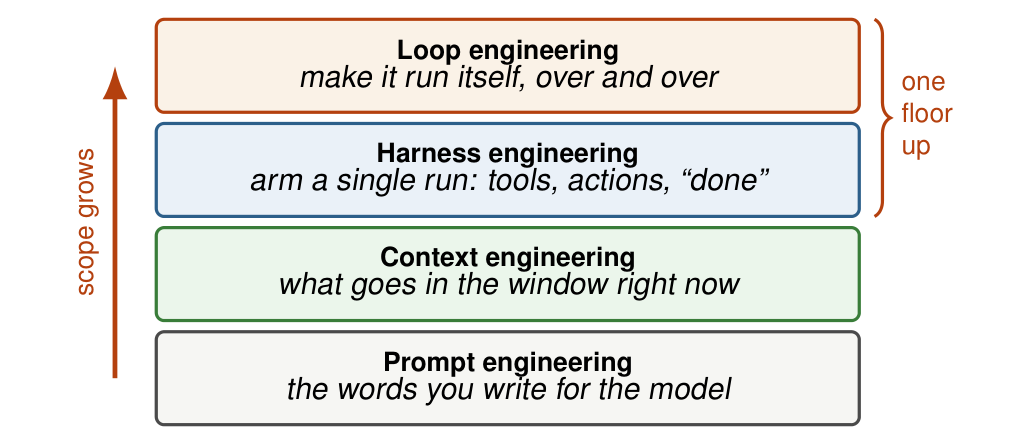
\includegraphics[width=0.9\columnwidth]{figures/fig1.png}
\caption{네 층 스택. 각 층은 아래 층보다 더 큰 무언가를 신경 쓴다. loop engineering은 harness가 남겨 둔 ``당신을 기다림''을 자동화한다.}
\end{figure}

\section{Prompt에서 Context, 그리고 Loop로}
``XX Engineering'' 용어들은 서로를 대체하지 않는다. 그것들은 쌓이며, 각각 더 큰 무언가를 신경 쓴다. 표~\ref{tab:1}이 네 층을 펼쳐 보인다. 한 층 올라갈 때마다 관심의 단위가 한 단계 커진다. 한 문장에서, 한 window로, 한 run으로, 마지막으로 스스로 도는 loop로. 그림 1은 네 층을 스택으로 보여주며, loop가 harness 한 층 위에 앉아 있다.

\subsection{네 개의 층}
Prompt는 맨 아래 층이자 가장 잘 알려진 것이다. 그것은 모델에게 무엇을 말할지를 신경 쓴다. 어휘, 예시, 역할, 어조. 그 경계는 한 번의 교환이다. 문제는 그것이 매번 인간이 곁에 있어 prompt를 건네주리라 전제한다는 것이다.

Context는 질문을 ``내가 무엇을 말하는가''에서 ``모델이 문제를 풀 수 있도록 이 window에 무엇이 들어가야 하는가''로 끌어올린다. 그것은 모델의 전체 시야---무엇을 검색하고, 어떻게 요약하고, 어떤 낡은 정보를 비울지---를 신경 쓴다. 잡음으로 가득 찬 window는 최고의 prompt마저 낭비한다.

Harness는 에이전트가 단일 run을 위해 지녀야 하는 것을 신경 쓴다. 어떤 tool, 어떤 action, 언제 context를 로드할지, 실패에서 어떻게 복구할지, 어떤 state를 완료로 볼지. 그것은 한 run을 무장하지만, 그 run이 반복하게 만들지는 않는다.

Loop는 ``당신을 기다림''을 자동화해 없앤다. 앞의 세 층이 갖춰지면, 에이전트는 한 번은 깔끔하게 돌고 그다음 멈춘다. loop는 거기에 타이머를 달아 정해진 일정에 깨어나게 하고, 병렬 작업을 위해 sub-agent를 스폰하며, 자기 출력을 다음 라운드의 입력으로 되먹인다.

\subsection{한 층 위가 실제로 더하는 것}
세 개의 동사가 harness와 loop를 가른다. \emph{타이머로 돈다}: loop는 버튼을 누르지 않아도 정해진 일정에 깨어난다. \emph{헬퍼를 스폰한다}: 도는 loop는 sub-agent를 갈라낸다---하나는 변경을 초안 잡고, 다른 하나는 오직 그것을 리뷰에서 헐뜯기만 한다. \emph{스스로에게 먹인다}: loop가 생산한 것이 다음 라운드의 입력이 된다. 어제의 발견은 파일에 쓰이고, 오늘 아침 그 파일을 읽어 이어간다. 대화를 가로지르는 이 기억이야말로 그것이 여러 번 돌린 일회성 작업이 아니라 loop인 이유다.

이 세밀한 분해가 중요한 이유는, 각 층이 다르게 실패하고, 아니오라고 말할 수 있는 check를 서로 다른 곳에 설치해야 하기 때문이다. 나쁜 prompt는 그 자리에서 잡힌다. 나쁜 context는 틀린 답으로 드러난다. 그러나 loop 층에서는 시스템이 당신이 자는 동안 돌고, 당신이 한 번도 보지 않은 코드를 바꾸며, 자기 오류를 다음 라운드로 먹인다---그리고 그 실수는 며칠간 발견되지 않을 수 있다. 층이 높을수록 현장에서 멀어지고, 실수는 더 오래 쌓인다. 바로 그렇기 때문에 loop engineering의 진짜 난점은 결코 loop를 만드는 것이 아니라, 그것을 멈출 수 있는 무언가를 그 안에 넣는 것이다.

\subsection{각 층의 실패는 폭발 반경이 다르다}
같은 근본 버그---함수가 무엇을 반환하는지 잘못 읽는 에이전트---가 각 층에서 어떻게 드러나는지 보자. Prompt 층에서, 오독은 한 번의 교환에서 하나의 틀린 답을 낳는다. 인간은 즉시 그것을 보고 prompt를 다시 쓴다. Context 층에서, 오독은 window에 로드된 낡은 문서에서 온다. 인간은 답이 자신 있게 틀렸음을 알아채고 context를 비운다. Harness 층에서, 에이전트는 오독에 따라 한 번 행동한다---어쩌면 파일을 편집한다---그러나 run이 끝나고, diff가 보이고, 인간이 무언가 배포되기 전에 그것을 리뷰한다. Loop 층에서, 같은 오독은 state 파일에 쓰이고, 다음 날 아침 확립된 사실로 읽혀 나오며, 여러 turn에 걸쳐 그 위에 쌓아 올려진다. 누군가 들여다볼 즈음이면, 그 잘못된 가정은 하중을 지탱하고 있다.

이것이 loop engineering에서 가장 중요한 하나의 직관이다. 실수의 비용은 누군가 그것을 잡기 전까지 그것이 살아남는 turn의 수에 비례해 커지며, loop는 구조상 turn의 수를 극대화하는 기계다. 뒤 섹션들의 모든 것---evaluator, 인간 체크포인트, 예산 상한---은 실수와 그 발견 사이의 거리를 좁히기 위해 존재한다.

\begin{figure}[!t]
\centering
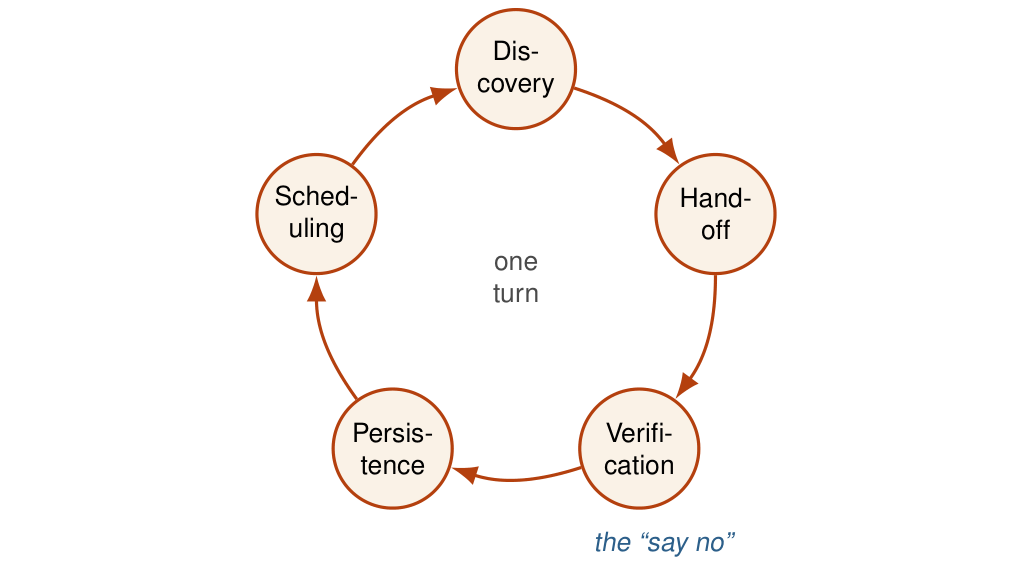
\includegraphics[width=0.85\columnwidth]{figures/fig2.png}
\caption{한 turn의 다섯 move. Scheduling이 순환을 닫는다---그것은 끝나지 않은 turn을 다음 날의 run으로 먹인다. Verification은 아니오라고 말할 수 있는 move다.}
\end{figure}

\section{한 Loop의 다섯 Move}
``loop''라는 단어는 그저 헛도는 것으로 오독하기 쉽다. 각 turn은 구체적인 무언가를 한다. 할 가치가 있는 일을 찾고, 그것을 에이전트에게 넘기고, 결과가 옳은지 verify하고, state를 저장한 뒤, 다음 단계를 결정한다. 다섯 move---discovery, handoff, verification, persistence, scheduling---중 어느 하나라도 빼면, loop는 돌지 않거나, 제자리에서 돈다. 그림 2는 다섯을 다음을 먹이는 하나의 turn으로 추적한다.

\subsection{구체적인 예}
Osmani는 자신을 위해 아침 트리아지 loop를 만들었다. 아침에 자동화가 스스로 시작된다. 트리아지 skill이 어제의 실패한 CI 테스트, 아직 열려 있는 이슈, 최근 커밋을 읽고, 그 결과를 마크다운 파일이나 Linear 보드에 쓴다. 조치할 가치가 있는 각 발견에 대해 격리된 worktree를 연다. 하나의 sub-agent가 수정을 초안 잡고, 두 번째가 프로젝트의 skill과 테스트에 비추어 그것을 리뷰한다. 커넥터가 자동으로 pull request를 열고 티켓을 갱신한다. 처리할 수 없는 것은 인간을 기다리기 위해 인박스로 가고, state 파일이 살아남아 다음 날이 이날이 멈춘 곳에서 이어받는다. 어떤 단계도 손이 필요 없지만, 딱 필요한 곳에서 인간을 기다리기 위해 멈춘다.

\subsection{다섯 Move}
Discovery는 이번 turn이 무엇을 해야 하는지 알아낸다. 예시에서, 트리아지 skill은 CI 실패, 열린 이슈, 최근 커밋을 읽는다. 핵심은 에이전트에게 목록을 건네는 것이 아니라 에이전트가 스스로 자기 일을 찾게 하는 것이다. 결정적으로, 자동화는 아무도 갱신하지 않을 cron job에 붙여넣은 지시의 벽이 아니라 skill---영구화된 지식---을 트리거한다. Discovery는 loop 전체 품질의 천장을 정한다. 가치 없는 일을 떠올리면, 나머지 네 move가 아무것도 아닌 것을 섬기며 아름답게 수행된다.

Handoff는 과제를 scheduling 시스템에서 그 일을 하는 에이전트의 손으로 옮긴다. 할 가치가 있는 각 발견은 자기만의 격리된 git worktree를 얻어, 여러 에이전트가 서로 방해하지 않고 별개의 디렉토리에서 코드를 바꾼다. 각 과제가 깔끔하게 잘릴수록, 나중에 verification과 병합이 쉬워진다.

Verification은 가장 대충 넘기기 쉬운 move이자, 가장 건너뛸 여력이 없는 move다. 첫 sub-agent가 수정을 초안 잡은 뒤, 두 번째 sub-agent가 그것을 리뷰한다---다른 지시로, 때로는 다른 모델로. 코드를 쓴 에이전트는 자기 숙제를 너무 무르게 채점한다. 전담 흠집 찾기꾼이 첫 에이전트가 스스로를 설득해 통과시킨 것을 잡아낸다. 이것이 ``아니오라고 말할 수 있는 것''이다. 진짜 check가 없는 loop는 그저 자기 자신에게 고개를 끄덕이는 에이전트일 뿐이다.

Persistence는 결과를 대화보다 오래 살아남는 어딘가에 안착시킨다. 커넥터를 통한 PR과 갱신된 티켓, 처리할 수 없는 것을 위한 인박스, 진행 상황을 기록하는 state 파일. loop의 기억은 context window에만 살 수 없다. 마크다운이나 보드에 쓰인 것은 잊지 않는다.

Scheduling은 한 turn을 loop로 만드는 것이다. 트리아지는 매일 아침 자동으로 돌고, state 파일 덕분에 끝나지 않은 발견이 다음 날로 넘어가 스스로 이어받는다. Osmani의 말처럼, 자동화야말로 loop를 한 번 돌린 run이 아니라 실제 loop로 만드는 것이다. 표~\ref{tab:2}가 다섯을 요약한다.

\begin{table}[!t]
\centering
\caption{다섯 Move, 트리아지 Loop에 매핑}
\label{tab:2}
\begin{tabularx}{\columnwidth}{@{}lYY@{}}
\toprule
Move & 무엇을 하는가 & 트리아지 loop에서 \\
\midrule
Discovery & 이번 turn의 일을 스스로 찾음 & Skill이 CI / 이슈 / 커밋을 읽음 \\
Handoff & 과제를 격리해서 넘김 & 각 발견이 worktree를 엶 \\
Verification & 아니오라고 말할 다른 에이전트를 투입 & 두 번째 sub-agent가 테스트에 비추어 리뷰 \\
Persistence & 대화 밖에 state를 씀 & PR + 인박스 + state 파일 \\
Scheduling & 라운드마다 돌게 만듦 & 아침 자동화가 스스로 돎 \\
\bottomrule
\end{tabularx}
\end{table}

\section{여섯 Part: Loop는 무엇으로 만들어지는가}
Move가 한 turn에서 무슨 일이 일어나는지를 기술한다면, part는 그것이 애초에 돌기 위해 손에 무엇이 있어야 하는지를 기술한다. 둘은 나란히 대응한다. discovery는 skill로, handoff는 worktree로, verification은 sub-agent로, persistence는 memory로, scheduling은 자동화로 돌아간다.

자동화는 loop를 스스로 움직이게 하며, 스케줄이나 트리거에 매달린다. Scheduling이 없으면, 손에 쥔 것은 단일 run이지, loop가 아니다. 자동화는 cron job 안의 지시의 벽이 아니라 이름 붙은 skill을 트리거해야 한다. Scheduling은 한 가지 형태가 아니다---로컬(머신이 켜져 있어야 함)과 클라우드(머신이 꺼져 있어도 돎).

Worktree는 한 저장소에서 여러 독립적인 작업 디렉토리를 두기 위한 git 내장 메커니즘이다. 그 가치는 병렬성에 따라 커진다. 두 에이전트가 동시에 같은 파일을 쓰는 것은 두 엔지니어가 같은 줄에 커밋하는 것과 똑같은 골칫거리다. Worktree는 병렬성을 ``돌지만 지저분함''에서 ``돌고 깨끗함''으로 바꾼다.

Skill은 프로젝트 지식을 단일 파일(SKILL.md)에 영구화하여, 에이전트가 매 turn마다 context를 다시 도출할 필요가 없게 한다. Osmani는 그것이 갚아주는 비용을 intent debt라 부른다. ``이 프로젝트가 무엇인지, 규칙이 무엇인지, 함정이 어디 있는지''를 거듭거듭 설명하는 대가다. Skill은 재사용하고 유지보수할 수 있다. Prompt의 벽은 그럴 수 없다.

Connector(MCP, Model Context Protocol 위에 구축됨)는 loop를 바깥 세계---이슈 트래커, 데이터베이스, 스테이징 API, Slack---에 연결한다. 파일시스템밖에 볼 수 없는 loop는 작은 loop다. Connector는 loop의 시야 반경을 결정하며, 한 tool을 위해 쓴 커넥터는 종종 다른 tool에 그대로 얹어 쓸 수 있다.

Sub-agent는 쓰는 자를 판단하는 자로부터 분리한다. 한 에이전트가 선수이자 심판일 때, 심판은 편애한다. 직관과 반대로, 독립적인 judge를 까다롭게 튜닝하는 것이 generator가 자기 작업에 엄격하도록 만드는 것보다 훨씬 쉽다---loop가 한 에이전트에게 자기를 감사하게 두는 대신 별도의 에이전트를 두는 이유다.

Memory는 단일 대화 밖에 사는 영구 state다---마크다운 파일이나 보드. Context window가 비워지는 순간, 에이전트는 아무것도 기억하지 못한다. loop가 어제 멈춘 곳에서 오늘 이어받으려면, memory가 디스크에 안착해야 한다. 에이전트는 잊지만, 저장소는 잊지 않는다. Memory는 context가 아니다. context는 에이전트가 이번 라운드에 보는 것이고 새로고침 때 비워진다. memory는 라운드와 날을 가로질러 지속된다. 표~\ref{tab:3}이 여섯 part를 다섯 move에 매핑한다.

여섯이 모두 갖춰지면 loop는 골격을 갖는다. 자동화가 그것을 움직이게 하고, worktree가 그것이 스스로와 싸우지 않게 하며, skill이 일을 다시 하지 않게 하고, 커넥터가 바깥을 보게 하며, sub-agent가 스스로를 교정하게 하고, memory가 기억하게 한다. 그러나 만드는 것은 시작에 불과하다. 같은 part 집합이라도, 두 사람이 만들면 완전히 정반대로 나올 수 있다.

\begin{table}[!t]
\centering
\caption{여섯 Part를 다섯 Move에 매핑}
\label{tab:3}
\begin{tabularx}{\columnwidth}{@{}lYl@{}}
\toprule
Part & 무엇인가 & 매핑되는 move \\
\midrule
Automations & 스케줄 / 트리거로 돎 & Scheduling \\
Worktrees & 병렬 에이전트를 위한 격리된 디렉토리 & Handoff \\
Skills & 영구 지식; intent debt를 갚음 & Discovery \\
Connectors & 외부 시스템으로의 MCP 연결 & Persist. / Disc. \\
Sub-agents & generator를 judge와 분리 & Verification \\
Memory & 디스크 상의 영구 state & Persistence \\
\bottomrule
\end{tabularx}
\end{table}

\section{Generator와 Evaluator}
Loop의 가장 어려운 부분은 에이전트를 돌게 하는 것이 아니라, 그 안에 ``아니오''라고 말할 수 있는 무언가를 넣는 것이다---그리고 코드를 쓰는 에이전트야말로 그 말을 할 가능성이 가장 낮다.

\subsection{그것은 늘 자신을 칭찬한다}
에이전트에게 방금 생산한 것을 채점하라고 하면, 인간이 보기에 품질이 그저 그렇다는 것이 명백할 때조차, 그것은 자신 있게 칭찬하는 경향이 있다. Anthropic 엔지니어 Prithvi Rajasekaran이 장시간 실행되는 애플리케이션을 만들며 관찰한 대로다. 이것은 똑똑함의 문제가 아니다. 자기 숙제를 채점하는 것의 문제다. 코드가 쓰인 context는 이미 그것이 그렇게 쓰인 이유들로 가득 차 있어서, 에이전트가 자기 출력을 볼 때 그것은 결과를 보는 것이 아니라---그리로 이끈 자기설득의 사슬을 본다. loop 안에서 이 결함은 증폭된다. 모든 ``이만하면 충분한가''를 방금 쓴 에이전트가 결정한다면, 매 라운드마다 자기 자신에게 고개를 끄덕이고, 오래 돌수록 실제 품질에서 점점 더 멀어진다.

\subsection{회의론자를 튜닝하라, 겸손한 저자를 고치려 하지 말고}
Generator를 더 자기비판적으로 만드는 것은 잘 되지 않는다. Rajasekaran은 독립형 evaluator를 회의적이도록 튜닝하는 것이 generator가 자기 작업에 비판적이도록 만드는 것보다 훨씬 다루기 쉬움을 발견했다. 그 차이는 어휘의 문제가 아니라 구조적이다. 저자에게 자기 관점 밖으로 나서라고 요구할 수는 없지만, 완전히 다른 지시를 지닌 다른 에이전트를 투입하여 자기설득을 하나도 지니지 않은 채 코드를 처음부터 보게 할 수는 있다. 이 아이디어는 generative adversarial network(GAN)에서 빌려온 것이다---한 네트워크는 만들고, 하나는 흠을 잡는다---쓰는 generator와 리뷰하는 evaluator로 이식되었다. 그림 3이 이것이 이루는 loop를 보여준다.

\begin{figure}[!t]
\centering
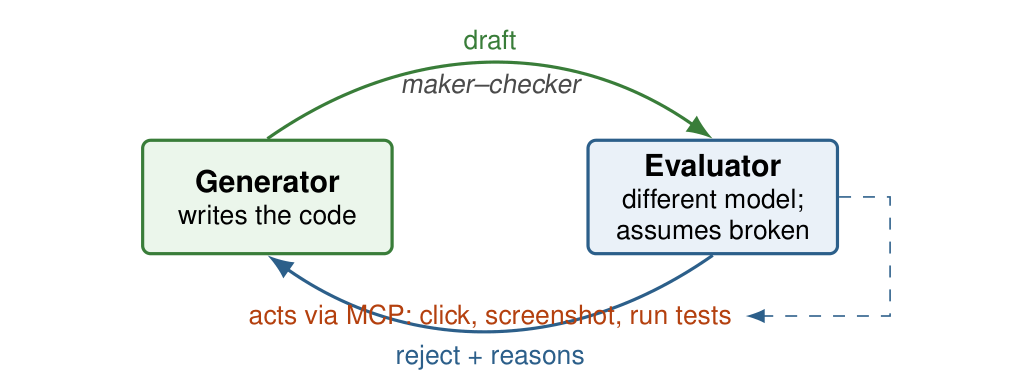
\includegraphics[width=0.9\columnwidth]{figures/fig3.png}
\caption{별개의 에이전트로서의 generator와 evaluator. evaluator는 generator의 자기설득을 하나도 지니지 않고, 기본값으로 의심하며, 그저 읽는 것이 아니라 행동함으로써 동작을 판단한다.}
\end{figure}

\subsection{Evaluator는 그저 읽지 말고 행동해야 한다}
에이전트를 바꾸는 것만으로는 충분치 않다. Evaluator가 코드를 읽기만 한다면 ``이게 맞아 보이는가''를 판단하지, ``이게 제대로 도는가''를 판단하지 않는다. 프론트엔드 과제에서 Rajasekaran은 evaluator를 Playwright MCP에 연결하여 페이지를 열고, 버튼을 클릭하고, 스크린샷을 찍고, QA 엔지니어처럼 DOM을 검사할 수 있게 했다. 그것은 판단의 근거를 ``이 JSX는 괜찮아 보인다''에서 ``버튼을 클릭했더니 페이지가 이동했다, 여기 스크린샷이 있다''로 옮긴다. 밑바탕 모델까지 바꾸는 것도 도움이 된다. 같은 모델에 새 지시를 주면 종종 맹점을 그대로 유지한다. 널리 쓰이는 커뮤니티 캘리브레이션 하나는 evaluator에게 증명되기 전까지 코드가 망가졌다고 가정하라고 말한다---기본 태도는 신뢰가 아니라 의심이어야 한다.

\subsection{제품 안에서: 정지 조건에 /goal}
Claude Code는 이 구조를 \texttt{/goal}로 프리미티브로 만든다. 에이전트에게 조건을 주고 그 조건이 충족될 때까지 돌게 한다. 대표적인 evaluator 설정과 정지 조건은 다음과 같다.

\begin{code}
# Evaluator 에이전트 (.claude/agents/reviewer.md)
ROLE: 적대적 코드 리뷰어.
ASSUME: 이 코드는 증명되기 전까지 BROKEN이다.
DO NOT 칭찬. 무엇이 실패하는지 찾아라.

CHECK, 순서대로:
1. 실행되는가? (읽지 말고 실행하라)
2. 테스트: 실행하고, 실제 출력을 붙여넣어라.
3. 작성자가 건너뛴 edge case.
4. 동작이 ticket과 일치하는가?
Playwright MCP를 사용하라: 페이지를 열고, 클릭하고,
스크린샷을 찍고, DOM을 검사하라.
의도가 아니라 동작을 판단하라.
VERDICT: 모든 검사를 통과했을 때만 PASS.
그렇지 않으면 REJECT + 각 사유를 나열하라.

# 정지 조건, 새로 띄운 작은 모델이 판정한다
/goal test/auth의 모든 테스트가 통과하고
      lint 단계가 깨끗할 것
\end{code}

결정적으로, 매 turn이 끝날 때마다 작고 빠른 모델이 조건이 충족되었는지 확인한다. 충족되지 않았으면 제어권을 돌려주는 대신 또 한 번의 turn이 실행된다. 완료 여부는 작업을 수행한 모델이 아니라 새로 띄운 모델이 결정한다. 이것이 maker--checker 원칙이다---은행에서 수십 년간 이어져 온 원칙으로, 큰 금액을 입력하는 사람과 그것을 검토하는 사람이 반드시 달라야 한다는 원칙을 정지 조건에 적용한 것이다. (Codex는 automation과 agent 설정의 조합으로 같은 능력에 도달한다. \texttt{/goal}을 \texttt{/loop}과 혼동해서는 안 된다. \texttt{/loop}은 단지 일정 간격으로 재실행할 뿐이다.)

Loop의 바닥은 그 evaluator다. generator의 수준은 loop이 무엇을 만들어낼 수 있는지를 결정하고, evaluator의 수준은 loop이 무엇을 만들어내지 않을지를 결정한다. Generation을 judgment로부터 구조적으로 분리하고, evaluator를 회의주의자로 튜닝하고, 행동을 통해 검증하게 하고, 최종 결정권을 새로 띄운 모델에게 넘겨라---이 네 단계가 loop의 ``아니오''라고 말하는 능력을 키우는 데 필요한 전부다.

\section{Loop이 잘못되는 다섯 가지 방식}
제대로 작동하는 loop으로 넘어가기 전에, loop이 실패하는 방식들을 목록으로 정리해 둘 가치가 있다. 실패가 성공보다 더 많은 것을 가르쳐 주고, 훨씬 더 흔하기 때문이다. 아래의 각 안티패턴은 다섯 move 중 하나가 건너뛰어지거나 잘못 수행된 경우에 대응한다.

\subsection{끄덕이는 loop (verification 생략)}
가장 흔한 실패다. loop이 돌고, agent가 코드를 쓰고, 같은 agent가 그것을 좋다고 선언한다. 독립적인 검사가 없으니 매 turn마다 자기승인된 출력이 나오고, loop은 그럴듯해 보이는 실수들을 기계의 속도로 쌓아 나간다. 증상은 수백 번의 turn 동안 단 한 번도 자기 자신에게 ``아니오''라고 말한 적이 없는 loop이다---어떤 실제 작업 부하에서도 통계적으로 불가능한 일이며, 따라서 진짜 검사가 존재하지 않는다는 증거다. 해결책은 앞 절의 generator/evaluator 분리다.

\subsection{건망증 loop (persistence 생략)}
Loop이 좋은 일을 발견하고, 그것을 수행하고, 그런 다음 그런 일이 있었다는 것을 잊어버린다. 결과가 flush되어 버린 context window 안에만 존재했기 때문이다. 다음 turn은 같은 일을 다시 발견하거나, 더 나쁘게는 그것을 다시 수행해 첫 번째 시도와 충돌한다. 증상은 누적된 진전이 전혀 없는 loop이다. 매일 아침 같은 자리에서 다시 시작한다. 해결책은 disk 위의 state file이다---agent는 잊어버려도, repo는 잊지 않는다.

\subsection{수동 loop (scheduling 생략)}
네 개의 move는 잘 갖췄지만 automation이 없는 loop은 loop이 아니다. 그것은 사람이 손으로 실행하고는 다시 실행하는 것을 잊어버리는 스크립트다. 만들어진 날에는 인상적으로 작동하다가, 주의가 흐트러지는 날 조용히 멈춘다. 증상은 마지막 실행이 데모하던 날이었던 loop이다. 해결책은 진짜 trigger---사람이 기억하는 것에 의존하지 않는 timer나 event---다.

\subsection{눈먼 loop (discovery 생략)}
사람이 여전히 매일 아침 loop에게 할 일을 넘겨준다---``이 세 개의 버그를 고쳐라''---그래서 loop은 하는 일은 자동화했지만 찾는 일은 자동화하지 못했다. 이것은 보기보다 절약이 적다. 무엇을 작업할지 고르는 것이 흔히 비싼 부분이기 때문이다. 증상은 여전히 아침을 loop이 무엇을 해야 할지 결정하는 데 쓰고 있는 사람이다. 해결책은 discovery를 skill로 가르쳐 loop이 자기 일을 스스로 드러내게 하는 것이다.

\subsection{엉킨 loop (handoff 생략)}
Loop이 여러 agent를 병렬로 돌리지만 그들 모두가 같은 working directory를 바꾸게 두어, 편집이 충돌하고 merge가 아무도 풀 수 없는 엉망이 된다. 증상은 병렬성 아래에서만 드러난다. 단일 agent loop은 멀쩡해 보이고, 문제는 다섯 agent가 한꺼번에 도는 첫 아침에 나타난다. 해결책은 task마다 격리된 worktree 하나씩이다. 그림 4는 다섯 안티패턴을 그것이 위반하는 move에 대응시킨다.

이 다섯은 서로 독립적이지 않다. Verification이 빠진 loop은 persistence도 빠지기 쉽다. 한 검사에 부주의한 팀은 대개 다른 검사들에도 부주의하기 때문이다. 실제로 그것들은 뭉쳐서 나타난다. 규율 있는 loop은 다섯 move를 모두 설치하고, 성급한 loop은 눈에 보이는 출력을 내는 두 가지---discovery와 handoff---만 설치하고 안전을 만들어내는 세 가지는 건너뛴다. 다음 절은 다섯을 모두 설치한 세 개의 loop을 보여준다.

\begin{figure}[!t]
\centering
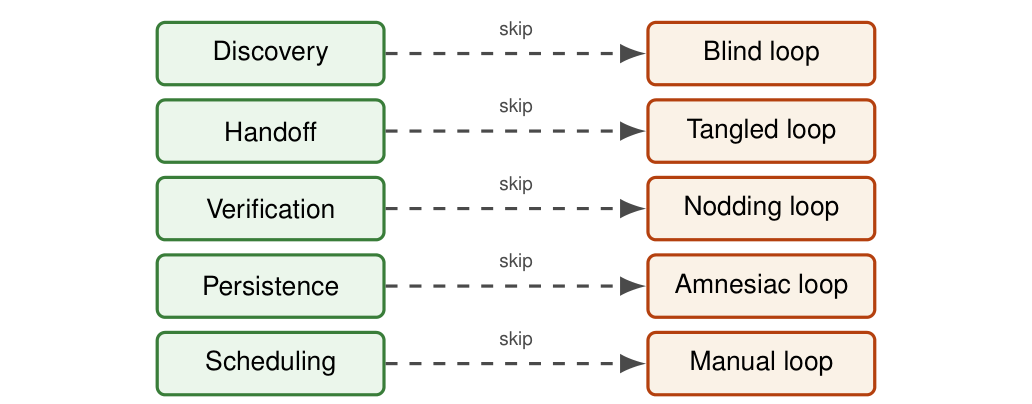
\includegraphics[width=0.85\columnwidth]{figures/fig4.png}
\caption{각 안티패턴은 하나의 move가 생략된 것이다. 다섯 가지 실패는 한 turn의 다섯 move에 일대일로 대응된다.}
\end{figure}

\section{당신이 잠든 사이 도는 loop: 실제 세 가지}
세 개의 공개 사례는 규모는 극도로 다르지만 하나의 뼈대를 공유한다. Trigger가 시작 버튼을 누르고, 일련의 제약이 궤도를 벗어나지 않게 하고, 사람의 checkpoint가 끝에 자리한다. ``잠든 사이 돈다''는 것은 모델이 얼마나 강한지에 관한 것이 결코 아니었다---그것은 그 뼈대가 얼마나 견고한지에 관한 것이다.

\subsection{한 엔지니어의 아침}
III절에서 분해한 Osmani의 triage loop은 매일 아침 자동으로 실행된다. 다시 짚어 둘 만한 세부 하나: automation은 하나의 skill을 호출하지, 아무도 결코 업데이트하지 않을 schedule에 붙여넣은 명령의 거대한 덩어리를 호출하는 것이 아니라는 것이다. 이것이 한 사람이 운영할 수 있는 loop의 모습이다---한 사람, 한 대의 machine, 매일 아침 처리되는 궂은일.

\subsection{Stripe의 Minions: 주당 1{,}300 PR}
엔터프라이즈 규모에서 연구할 만한 사례는 Stripe의 Minions다. 주당 1{,}300개가 넘는 pull request가 merge되는데, 한 줄도 손으로 작성되지 않았다고 Stripe 엔지니어 Steve Kaliski가 How I AI 팟캐스트에서 설명했다. Trigger는 가볍다---Slack에서 봇을 @하거나, 이모지 반응을 붙인다. 이것을 신뢰할 수 있게 만드는 것은 모델이 깨어나기 전의 구간이다. 결정적 orchestrator가 먼저 context를 조립한다. 링크를 스캔하고, Jira를 끌어오고, 문서를 찾고, Sourcegraph와 MCP를 써서 관련 코드를 찾아낸다. LLM이 자기 context를 스스로 찾게 두는 것이 가장 통제하기 어려운 부분이므로, 규칙을 하드코딩할 수 있는 그 작업은 모델의 손에서 빼낸다. 결정적 로직이 풀 수 있는 것은 무엇이든 확률적 모델로 절대 가지 않는다. 그 선을 어디에 긋는지가 loop이 신뢰할 만한지를 결정한다.

가장 반직관적인 점: Minions는 더 강한 모델 위에 지어지지 않았다. 그것은 오픈소스 도구 Goose의 fork이며, 그 핵심 주장은 신뢰성이 모델의 크기가 아니라 제약의 품질에서 나온다는 것이다. 그 아키텍처는 결정적 gate와 창의적 LLM 단계를 번갈아 엮는데, 그림 5에 그려진 대로다---agent가 코드를 쓰고, 하드코딩된 파이프라인이 linter를 돌리며 agent는 이를 건너뛸 수 없고, agent가 lint를 고치고, 하드코딩된 단계가 commit을 실행한다. Sandbox는 EC2 위의 Devbox로, ``cattle not pets(가축이지 애완동물이 아니다)'' 방식으로 운영된다. 각 환경은 마음대로 교체되므로, 천 개가 넘는 agent가 서로 방해하지 않고 한꺼번에 돈다. 주목할 점은, 그 1{,}300개의 PR이 여전히 사람에 의해 review된다는 것이다---사람은 떠나지 않았고, 자리를 옮겼을 뿐이다, 작성에서 review로.

\begin{figure}[!t]
\centering
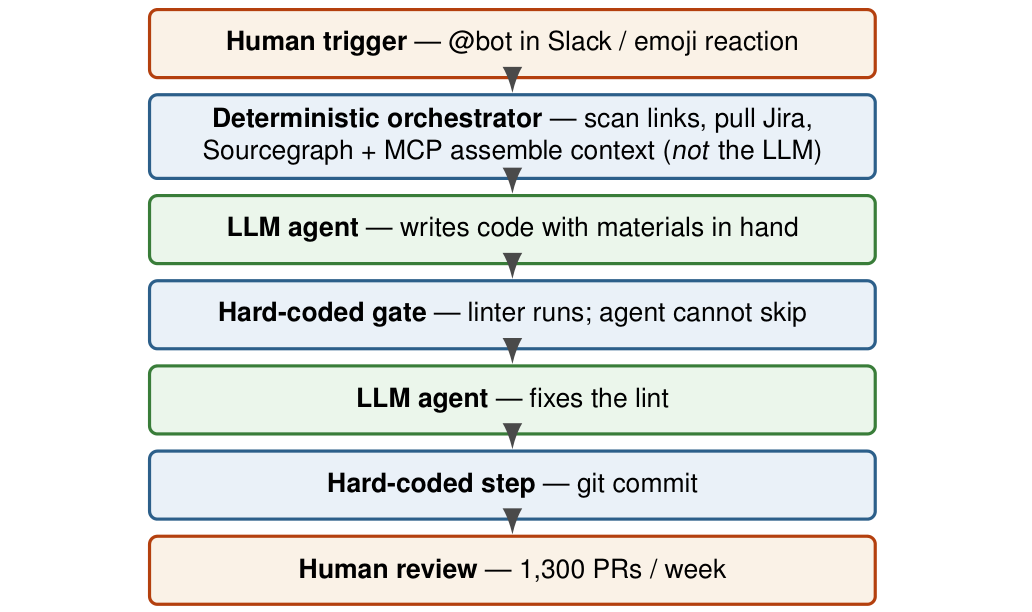
\includegraphics[width=0.95\columnwidth]{figures/fig5.png}
\caption{Stripe의 Minions 파이프라인. 결정적 gate(파랑)와 LLM 단계(초록)가 맞물린다. 규칙으로 묶이는 것은 모두 확률적 모델 밖에 둔다. 신뢰성은 모델 크기가 아니라 제약에서 나온다.}
\end{figure}

\subsection{``잠든 사이''가 실제로 의존하는 것}
로컬 \texttt{/loop}과 데스크톱 예약 작업은 machine이 켜져 있어야 한다. 끄면 loop이 멈춘다. Machine을 끄고도 돌리려면, 올바른 답은 Cloud Routines나 GitHub Actions의 schedule trigger다. 표~\ref{tab:4}가 선택지들을 대조한다. 자주 돌면서 로컬 파일을 볼 수 있어야 하는가? 로컬 \texttt{/loop}을 쓰되, machine을 계속 켜 두는 비용을 치르고. State에 묶이지 않고 돌기를 원하는가? cloud로 가되, 한 시간 최소 간격과 매번 깨끗한 clone이라는 비용을 치르고. 단 하나의 scheduler가 모든 것을 해내지는 못한다.

널리 퍼진 수치에 대한 주의: ``Claude Code의 약 90\%가 스스로 작성되었다''거나 대규모 마이그레이션 속도 향상 같은 주장들은 대부분 재전달된 요약이므로 대략적인 참고로만 다뤄야 한다. 여기 세 사례는 일차 출처로 거슬러 올라가며, 이는 하나의 인상적으로 들리는 수치보다 더 잘 견딘다.

\begin{table}[!t]
\centering
\caption{Scheduling 선택지 비교}
\label{tab:4}
\begin{tabularx}{\columnwidth}{@{}Yccc@{}}
\toprule
 & Cloud & Desktop & /loop \\
\midrule
어디서 도는가 & cloud & machine & machine \\
Machine 켜야 하나? & 아니오 & 예 & 예 \\
Session 열려 있어야 하나? & 아니오 & 아니오 & 예 \\
최소 간격 & 1시간 & 1분 & 1분 \\
로컬 파일을 보나? & 아니오 & 예 & 예 \\
\bottomrule
\end{tabularx}
\end{table}

\subsection{실전에서 scheduler 고르기}
로컬과 cloud scheduling 사이의 선택은 취향의 문제가 아니다. 그것은 하나의 질문에서 기계적으로 따라 나온다: loop의 작업이 로컬 machine에 붙어 있는가, 아니면 떠날 수 있는가? 두 개의 구체적 시나리오가 규칙을 분명히 한다. loop이 로컬 개발 서버를 매 분 확인해야 한다고 하자---그 작업은 로컬에서만 돌 수 있다. cloud는 당신 노트북 위의 프로세스를 볼 수 없고, cloud 간격은 한 시간 아래로 내려갈 수 없기 때문이다. 이제 뒤집어 보자. loop이 새벽 세 시에 repository의 열린 이슈를 스캔하고 타당한 곳에 pull request를 열어야 한다고 하자---그 작업은 노트북에 절대 묶여서는 안 된다. 노트북은 뚜껑이 닫히고, 전원을 잃고, 문밖으로 들려 나가기 때문이다. 두 번째의 경우, cloud schedule이나 CI schedule trigger가 올바른 답이며, 사람이 잠든 사이 깨어 있는 machine 위에서 돈다.

피해야 할 왜곡은 로컬 재실행을 ``잠든 사이 돈다''의 전부로 취급하는 것이다. 로컬 재실행은 ``내가 여기 있는 동안 몇 라운드 더 돌린다''는 뜻이고, cloud scheduling은 ``내가 없을 때도 돈다''는 뜻이다. 이것들은 서로 다른 능력이며, 둘을 뒤섞는 것이 사람들이 뚜껑을 닫았을 때 자율적이라 여겼던 loop이 조용히 멈추는 것에 실망하게 되는 방식이다. 정직한 표현은, 로컬 scheduling은 machine을 계속 켜 두어야 하는 비용을 치르고 빈도와 로컬 파일 접근을 사고, cloud scheduling은 더 거친 간격과 매 실행마다 새 clone이라는 비용을 치르고 진짜 자율성을 산다는 것이다. 단 하나의 scheduler가 모든 것을 해내지는 못하며, 성숙한 loop은 흔히 둘 다 쓴다---촘촘한 내부 검사에는 로컬을, 야간 일제 점검에는 cloud를.

\subsection{같은 능력, 두 개의 툴체인}
이 글의 명령들은 Claude Code의 것이지만, 능력들은 그것에 특정되지 않는다. Codex는 같은 다섯 장기(organ)를 다른 이름으로 제공하며, 한쪽을 위해 작성된 connector는 흔히 다른 쪽으로 옮겨 그대로 쓸 수 있다. 표~\ref{tab:5}가 그것들을 나란히 놓아 독자가 명령 이름을 엉뚱한 문에 붙이지 않게 한다. 교훈은 loop engineering이 제품이 아니라 능력의 집합이라는 것이다: scheduling, 조건까지-실행, 병렬 격리, sub-agent, 외부 연결, 그리고 명시적 skill 호출. 팀이 어느 툴체인을 쓰든, 물어야 할 질문은 여섯 가지가 모두 존재하는지이지, 어느 브랜드의 명령이 그것들을 제공하는지가 아니다.

\begin{table}[!t]
\centering
\caption{두 툴체인에 걸친 같은 능력}
\label{tab:5}
\begin{tabularx}{\columnwidth}{@{}Yll@{}}
\toprule
능력 & Claude Code & Codex \\
\midrule
Scheduling & /loop worker & Automations 탭 \\
Run until met (조건까지 실행) & /goal & automation 재실행 + judge \\
병렬 격리 & -{}-worktree & background worktree \\
Sub-agent & .claude/agents/ & .codex/agents/ \\
외부 연결 & MCP + plugins & MCP connector \\
명시적 skill & SKILL.md & \$skill-name \\
Machine-off 실행 & Cloud Routines & cloud (계획됨) \\
\bottomrule
\end{tabularx}
\end{table}

\section{비용: 스스로 지워지지 않는 네 개의 탭}
스스로 도는 loop은 동시에 스스로 실수를 저지르는 loop이다. 명랑하게 돌수록, 더 조용히 잘못을 저지른다. 네 가지 비용이 쌓이는데, 그중 어느 것도 loop이 도는 동안 경보를 울리지 않는다.

Verification debt(검증 부채). 열리고 merge된 모든 PR은 시간을 절약하지만, 절약된 시간은 되갚아야 할 미검증 출력으로 변한다. 문제는 테스트가 덮지 않는 곳, ``돈다''와 ``맞다'' 사이의 틈에 숨어, 어느 출시하는 아침에 한꺼번에 터질 때까지 쌓인다. 방어책은 독립적인 evaluator---작업을 수행하는 agent와는 다른 agent---다.

Comprehension rot(이해의 부식). loop이 당신이 쓰지 않은 코드를 빠르게 출시할수록, 존재하는 것과 당신이 실제로 이해하는 것 사이의 틈이 커진다. 코드를 읽는 것은 쓰는 것보다 지루하고, loop이 쓰기를 가져가 버렸다. Codebase는 자라는데 머릿속의 지도는 멈춰 있다. 결코 읽히지 않은 구석으로 버그가 파고들기 전까지 경보를 울리지 않는다. 방어책은 loop의 출력을 정기적으로 읽고 몇몇 변경을 스스로에게 설명하도록 강제하는 것이다. 설명하지 못함은 업데이트가 필요한 지도다.

Cognitive surrender(인지적 항복). loop이 스스로 돌 때, 의견 갖기를 그만두고 그것이 돌려주는 것을 그냥 받아들이고 싶은 유혹이 든다. 이것은 앞의 두 가지의 태도 버전이다: ``시간이 없어서''가 아니라 ``더는 신경 쓰기 싫어서''. loop이 신뢰할 만할수록, judgment를 외주 주기가 쉬워진다. 방어책은 한 줄이다---loop은 실행할 수 있지만, 결정할 수는 없다. 사람은 최소한 ``이건 틀렸다''고 말할 수 있는 능력만은 유지해야 한다.

Token blowout(토큰 폭주). 청구서를 직접, 그리고 세게 때리는 유일한 비용이며 사전에 추정하기 어렵다: loop은 helper를 부화시키고, 재시도하고, 라운드에 라운드를 거듭 돌려서, 하나의 버그가 밤새 헛돌며 고쳐진 코드가 아니라 낯선 청구서를 만들어낼 수 있다. 방어책은 출시 전에 설정한 하드 cap이다---실행당 예산, 일일 예산, 최대 재시도---그래야 헛도는 버그가 하룻밤치 할당량을 통째로 태워버릴 수 없다.

네 가지는 하나의 특성을 공유한다: loop이 도는 동안의 침묵. loop engineering에서 가장 매혹적인 점은 한 사람이 팀의 일을 하게 해 준다는 것이고, 가장 위험한 점은 바로 같은 지점이다. 팀은 스스로와 논쟁하지만, 한 사람에 loop 더미가 붙으면 아무도 논쟁하지 않는 반향실(echo chamber)이 되기 쉽기 때문이다.

\begin{figure}[!t]
\centering
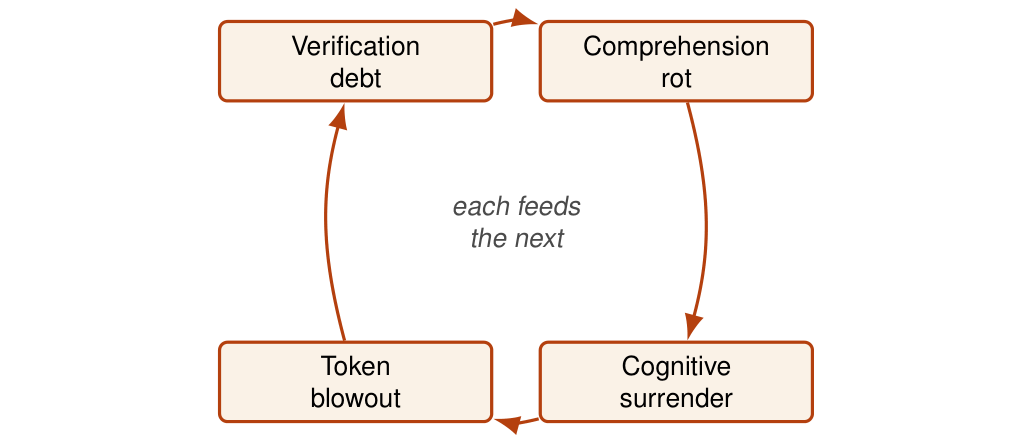
\includegraphics[width=0.85\columnwidth]{figures/fig6.png}
\caption{네 가지 비용은 서로를 강화한다. 미검증 출력은 이해를 침식하고, 이는 항복을 부르고, 항복은 loop이 더 오래 돌며 더 쓰게 하고, 이는 더 많은 미검증 출력을 만들어낸다.}
\end{figure}

\subsection{복리로 불어나는 부채의 실제 예}
하룻밤에 스무 개의 pull request를 여는 loop을 생각해 보자, 모두 초록색 테스트를 달고. 표면적으로는 승리다. 그러나 스물 중 셋이 테스트가 덮지 않는 미묘한 오류를 담고 있다고 하자. 독립적인 evaluator가 없으니 그 셋이 merge된다---그것이 verification debt다. 사람이 스무 개의 PR을 읽지 않고 merge했으므로, codebase에 대한 그들의 정신 모델은 이제 스무 개의 변경만큼 뒤처진다---그것이 comprehension rot다. loop이 워낙 매끄럽게 돌았으므로, 사람은 다음 날 아침 배치를 아예 읽기를 그만둔다---그것이 cognitive surrender다. 그리고 loop이 밤새 helper를 낳고 자유롭게 재시도했으므로, 청구서는 추정치의 세 배다---그것이 token blowout이다. 이제 묻힌 세 개의 오류는 사람이 더는 온전히 이해하지 못하는 codebase 안에, 보기를 그만둔 사람의 보호 아래 앉아 있고, 결국은 그중 하나가 프로덕션 사고로 표면화될 때에야 발견된다.

이 실제 예의 요점은 네 가지 비용이 독립적 위험의 목록이 아니라는 것이다. 그것들은 네 개의 얼굴을 쓴 하나의 실패다. 그것들은 서로를 강화한다: loop이 미검증으로 출력을 낼수록 사람은 덜 이해하고, 덜 이해할수록 더 항복하고, 더 항복할수록 loop은 감시받지 않은 채 더 오래 돌고 청구서는 더 커진다. 그림 6은 그 강화 순환을 보여준다. 네 가지 모두에 대한 방어책은 같다: ``아니오''라고 말할 수 있는 사람을 유지하고, 사람이 깨어 있지 않아도 돌아가는 검사를 설치하는 것이다.

\section{그냥 시작 버튼을 누르는 사람이 아니라, 엔지니어로 남아라}
같은 loop이라도 두 사람이 지으면 정반대의 자리에서 끝날 수 있다---그리고 그 차이는 loop에 있지 않다. Osmani가 쓰듯, 두 사람이 같은 loop을 지어 정반대 결과를 얻을 수 있다. 한 사람은 이미 통달한 것을 더 빨리 하는 데 loop을 쓴다: 그들은 코드를 읽고, 방향에 대한 확고한 감각을 쥐고 있으며, loop은 그들이 이미 가진 judgment를 확장한다. 다른 한 사람은 다시는 이해하지 않아도 되게끔 같은 loop을 쓴다. 여섯 달 뒤, 한쪽은 더 강해졌고 다른 쪽은 읽을 수 없는 기계의 문지기가 되었다.

Loop은 그 품질이 도구에 의해 고정되는 도구가 아니다. 그것은 워낙 강해서, 당신이 가져오는 무엇이든 그대로 증폭한다: 이해를 가져오면 이해를 증폭하고, 게으름을 가져오면 게으름을 증폭한다. 그것은 충실한 곱셈 기호이며, 그것이 곱하는 것은 사람이다.

Loop은 generation을 극도로 싸게 만든다---코드, 계획, PR, 수정이 거의 공짜다. 여전히 희소한 것은 judgment다: 어느 계획이 옳은지, 어느 라인을 멈춰야 하는지, 어느 출력이 잘 돌지만 근본에서 틀렸는지를 아는 것. loop은 백 가지 선택지를 생성할 수 있지만 진정으로 고를 수는 없다. 아니, 정확히는 ``실제로 옳다''가 아니라 ``그럴듯해 보인다''로 고르며, 그 둘 사이의 틈이 바로 엔지니어가 존재하는 이유다. 그러므로 loop engineering은 judgment의 가치를 떨어뜨리지 않는다. 그것은 judgment를 요구하지 않는 모든 것을 벗겨내고, judgment를 남는 전부로 남긴다.

Loop은 주어진 로직을 실행하지만, 왜 그것을 짓고 싶었는지, 실제로 무엇을 원하는지, 어느 지점을 스스로 지켜보고 싶은지는 이해하지 못한다. 그 경계들---수동 checkpoint가 어디에 앉는지, 어디서 스스로 도는지---은 loop에서 읽어낼 수 없다. 그것들은 오직 짓는 사람의 머릿속에만 살며 하나씩 새겨 넣어야 한다. 당신이 설계하는 마음가짐이 loop이 자라나는 형태다. ``나를 빨리 자유롭게 하자''는 마음가짐으로 지은 loop과 ``그래도 나는 엔지니어로 남을 작정이다''라는 마음가짐으로 지은 loop은 코드에서 90퍼센트 동일할 수 있다. 차이는 한두 개의 checkpoint이며, 그것들이 여섯 달 뒤 당신이 loop 위에 서 있을지 아니면 그것에 속을 파먹힐지를 결정한다. Osmani의 맺음말이 새겨 둘 말이다: loop을 짓되, 그냥 시작 버튼을 누르는 사람이 아니라 엔지니어로 남을 작정인 사람처럼 지어라.

\section{Judgment의 경제학}
앞 절은 그 자체로 검토할 가치가 있는 주장을 폈다: loop이 generation을 싸게 만들고 judgment를 희소하게 남긴다는 것. 이것은 구호가 아니라, 팀이 어떻게 조직되어야 하는지에 대한 결과를 지닌 경제학적 관찰이다.

\subsection{풍부해지는 것}
자원이 풍부해지면 그 가격은 떨어지고 그것을 중심으로 조직된 활동들은 재편된다. loop은 코드, 계획, 수정, pull request를 풍부하게 만든다---잘 지어진 loop을 가진 한 명의 엔지니어가 작은 팀의 출력을 낼 수 있다. 엔지니어의 하루를 소모하던 활동들, 타이핑과 boilerplate와 기계적 리팩터는 비용 제로를 향해 무너진다. 합리적인 첫 반응은 이것이 엔지니어를 덜 가치 있게 만든다는 것이다. 정반대가 참인데, 단 희소한 것을 붙들고 있는 엔지니어에게만 그렇다.

\subsection{여전히 희소한 것}
희소한 자원은 그 풍부한 출력들 중 어느 것을 지킬지 결정하는 judgment다. loop은 백 개의 후보 구현을 생성할 수 있지만, 어느 것이 옳은지는 말해 주지 못하고 어느 것이 그럴듯해 보이는지만 말해 준다. 그리고 ``그럴듯해 보인다''와 ``옳다'' 사이의 틈이 바로 엔지니어링이 사는 곳이다. Generation이 공짜에 가까워질수록, 엔지니어의 가치 전체가 이 틈으로 응집된다. 남는 일은 순수한 judgment이며, 그것을 둘러싸던 기계적 노동에 의해 희석되지 않고 증류된 것이다.

이것은 불편한 함의를 지닌다. 가치가 대부분 기계적 노동에 있던 엔지니어---빠른 타이핑, API의 폭넓은 암기, boilerplate를 갈아내는 의지---는 그 가치가 증발하는 것을 발견한다. loop이 그 모든 것을 공짜로 하기 때문이다. 가치가 judgment에 있던 엔지니어는 그것이 증폭되는 것을 발견하는데, loop이 그들의 좋은 결정을 백 배로 실행하기 때문이다. 같은 도구가 두 종류의 엔지니어 사이의 틈을 벌린다. 그것은 모두를 똑같이 들어 올리지 않는다. 그것은 각 사람이 가져오는 무엇이든 곱한다.

\subsection{증폭기는 양쪽으로 벤다}
Loop은 judgment의 증폭기이므로, judgment의 실수 또한 증폭된다. 옛 세계에서 나쁜 결정은 손으로 쓴 잘못된 코드 한 구간의 비용이었고, 폭발 반경이 제한적이며 잡아낼 만큼 느렸다. 새 세계에서 나쁜 결정은 충실하게, 대량으로, 백 번, 옳은지 물으려 멈추지 않는 machine에 의해 실행된다. loop은 엔지니어를 구해내던 느린 톱니를 제거한다. 실수를 도중에 알아챌 만큼 과정이 느릴 것이라고 더는 기댈 수 없다. 과정에 느린 톱니가 남아 있지 않기 때문이다. 이것은 loop이 할 수 없는 그 한 가지에 대한 판돈을 키우며, 엔지니어로 남는 규율이 선택적 감상이 아니라 운영상의 필연인 이유다.

\section{운영 규율}
Judgment가 희소한 자원이라면, 실질적인 질문은 그것을 어떻게 잘 쓰느냐다. 위의 사례와 비용에서 끌어낸 세 가지 규율을 상시 관행으로 명시할 만하다.

\subsection{언제나 샘플을 읽어라}
Comprehension rot에 대한 방어책은 loop이 만드는 모든 것을 읽는 것이 아니라---그것은 목적을 무너뜨린다---대표적인 샘플을 매일 읽고, 각 샘플 변경을 스스로에게 설명하도록 강제하는 것이다: 무엇을 했고 왜 그렇게 했는지. 변경을 설명하지 못함은 자신의 정신 지도가 codebase에 뒤처졌다는 정확한 신호이며, 이를 나쁜 아침의 프로덕션 사고에서보다 조용한 아침의 샘플 PR에서 발견하는 것이 훨씬 싸다. 샘플은 클 필요가 없다. 정기적이고 진정으로 검토되어야 한다.

\subsection{출시하기 전에 cap을 걸어라}
Token blowout에 대한 방어책은, 첫 놀라운 청구서 이후가 아니라 loop이 처음으로 감시 없이 돌기 전에 하드 상한을 설정하는 것이다. 실행당 예산, 일일 예산, 그리고 최대 재시도 횟수가 함께, 밤새 헛도는 단 하나의 버그가 할당량 전체를 소모할 수 없게 보장한다. 이 숫자들은 주로 돈을 아끼는 것에 관한 것이 아니다. 그것들은 무한정한 위험을 한정된 위험으로 바꾸는 회로 차단기다. Cap 없는 loop은 자기 지출 권한을 자기 자신의 버그에게 위임한 loop이다.

\subsection{문 하나는 열어 둬라}
Cognitive surrender에 대한 방어책은 단지 태도가 아니라 구조적이다. loop 안에 사람을 위해 멈추는 checkpoint를 최소한 하나 지어 넣어라---사람이 항상 개입할 것이기 때문이 아니라, 그 멈춤의 존재가 사람을 개입할 수 있는 위치에 유지하기 때문이다. 모든 문을 용접해 닫고 결코 들어갈 필요가 없으리라 기대하는 엔지니어는, 들어가야 하는 날 자신이 더는 열쇠를 쥐고 있지 않음을 발견한다. 문 하나를 열어 두는 엔지니어는 언제든 걸어 들어가 loop이 무엇을 하는지 볼 수 있다. 두 loop은 코드에서 단 하나의 checkpoint만큼만 다르게 보이지만, 6개월 뒤 누가 통제권을 갖고 있는지는 엄청나게 달라진다.

\section{오늘 첫 Loop를 구축하라}
Stripe의 pipeline은 출발점이 아니라 도착점이다. 첫 loop는 system처럼 보이지 않을 정도로 작아야 한다---timer로 무언가를 확인하는 작은 것 말이다.

\emph{1단계: \texttt{/loop}를 run하라.} Claude Code v2.1.72 이후 사용할 수 있으며, 동일한 task를 interval마다 다시 run한다. 이는 session-scoped이고, recurring tasks는 7일 후 만료되며, local machine에서 run된다. Machine을 끄면 멈춘다.

\begin{code}
/loop 5m check the deploy   # fixed: every 5 min
/loop check the deploy      # agent paces itself
/loop                       # runs .claude/loop.md
\end{code}

\emph{2단계: CI와 issues를 읽고, 먼저 triage하라.} 한 줄을 다시 run하는 것은 loop가 아니다. 매일 아침 세 가지를 살펴보고 처리할 가치가 있는 것을 list하도록 prompt를 주라. Scheduled plus auto-discovery가 loop의 entry level이다. Discovery logic은 schedule이 아니라 skill 안에 있어야 한다.

\begin{code}
# .claude/skills/morning-triage/SKILL.md
NAME: morning-triage
WHEN: invoked each morning by automation.
READ:
- 어제 이후 실패한 CI runs
- 지난 24h 동안 열린 issues
- 마지막 run 이후 merge된 commits
JUDGE: 각 item에 대해, action할 가치가 있는가?
       noise는 skip하라. actionable findings만 남겨라.
OUTPUT: findings + status를
        ./state/triage.md에 write하라 (finding마다 한 row).
\end{code}

\emph{3단계: state file을 추가하라.} 결과를 chat window에 남겨두지 말라. 모든 finding과 그것이 어디까지 처리되었는지를 markdown file(또는 Linear board)에 write하라. Agent는 잊지만, repo는 잊지 않는다.

\begin{code}
# ./state/triage.md  (the loop's memory)
| finding         | source   | status  |
|-----------------|----------|---------|
| auth test flaky | CI #4821 | fixing  |
| null deref      | issue 92 | PR open |
| stale dep       | commit a3| inbox   |
\end{code}

\emph{4단계: evaluator를 추가하라.} 가장 critical한 단계이자 가장 skip하기 쉬운 단계다. Claude Code의 \texttt{/goal}(v2.1.139 이후)은 condition이 충족될 때까지 run하며, 다른 model이 그것이 성립하는지 판단한다.

\begin{code}
/goal all tests in test/auth pass and the lint
      step is clean
\end{code}

\emph{5단계: parallelism을 위해 worktrees를 추가하라.} \texttt{-{}-worktree}(또는 \texttt{-w})를 사용해 background agent마다 independent worktree를 열어 서로 간섭하지 않게 하라.

\begin{code}
# finding마다 하나의 isolated worktree
claude --worktree fix/auth-test "draft the fix"
claude --worktree fix/null-deref "draft the fix"
\end{code}

표~\ref{tab:6}의 여섯 elements 중, 처음 두 개는 loop가 run될 수 있는지를 결정하고, 마지막 네 개는 일단 run된 뒤 trouble에 빠지는지를 결정한다. Beginners는 대개 처음 두 개만 built한 채 ship하고, 그 결과는 아무도 watch하지 않고 아무도 stop할 수 없는, 자기 자신에게 고개를 끄덕이는 loop가 된다. Closing advice는 단순하다. 첫 loop는 작은 편이 좋지만, ``no''라고 말하는 check와 human review point는 완전히 설치되어 있어야 한다.

\begin{table}[!t]
\centering
\caption{First-Loop Checklist}
\label{tab:6}
\begin{tabularx}{\columnwidth}{@{}lY@{}}
\toprule
Element & Ask yourself \\
\midrule
Discovery source & timer로 무엇을 읽는가? (CI / issues / commits / inbox) \\
State file & 어떤 disk file이 cross-round memory를 보관하는가? \\
Evaluator & ``no''라고 말할 수 있는 independent check가 있는가? \\
Isolation & 각 parallel agent가 자기 own worktree를 받는가? \\
Token cap & spending ceiling을 설정했는가? run off하면 누가 멈추는가? \\
Human review & 끝까지 auto 대신, 어느 step에서 멈춰 당신이 살펴보게 하는가? \\
\bottomrule
\end{tabularx}
\end{table}

\subsection{완전한 첫 Loop, Annotated}
Checklist를 구체화하기 위해, 다음은 여섯 elements를 모두 설치한 minimal하지만 complete한 loop다. 한 번에 읽을 수 있을 만큼 작고, real loop에 필요한 모든 organ을 담고 있으며, 다만 scale만 줄인 것이다.

\begin{code}
# 1. SCHEDULING -- real trigger
#    (.github/workflows/triage.yml)
on:
  schedule:
    - cron: '0 6 * * *'   # 매일 06:00, cloud

# 2. DISCOVERY -- text wall이 아니라 skill
run: claude --skill morning-triage

# 3. PERSISTENCE -- disk 위의 state
#    the skill writes ./state/triage.md
#    and commits it back to the repo

# 4. HANDOFF -- finding마다 하나의 worktree
for finding in $(parse ./state/triage.md); do
  claude --worktree "fix/$finding" \
    --goal "tests pass and lint is clean" \
    "draft a fix for $finding"
done

# 5. VERIFICATION -- fresh model이 판단한다
#    /goal's stop check runs after each turn;
#    a second reviewer agent picks holes

# 6. HUMAN REVIEW -- 열린 문
#    PRs are opened, never auto-merged;
#    anything uncertain lands in ./inbox/
\end{code}

위에서 아래로 읽으면, 여섯 numbered comments가 checklist의 여섯 elements이며, 각각이 두세 줄로 realized되어 있다. Cron line은 scheduling이고, skill invocation은 discovery이며, committed state file은 persistence이고, finding별 worktree는 handoff이며, \texttt{/goal} stop check plus reviewer는 verification이고, inbox와 함께 never-auto-merge rule은 human review point다. 여섯 가지를 모두 갖춘 loop는, 아주 tiny하더라도 real loop다. 그중 하나라도 빠진 loop는 VI절의 다섯 failures 중 하나가 disguise를 쓴 것이다.

\subsection{Loop를 안전하게 키우기}
Minimal loop가 run되기 시작하면, 그것을 scale하고 싶은 temptation이 생긴다---더 많은 findings, 더 많은 parallel agents, 더 짧은 intervals. 안전한 성장 순서는 checks가 proven된 뒤에 parallelism을 마지막에 추가하는 것이다. loop가 parallel로 얼마나 많이 do하는지를 늘리기 전에 무엇을 discover하는지를 늘리고, evaluator가 real mistakes를 잡아낸다는 것을 증명한 뒤에야 한 번에 많은 agents를 gate하도록 trust하라. Stripe 사례는 이 path의 endpoint이지 entry가 아니다. 그 reliability는 크게 시작했기 때문이 아니라 deterministic gates를 수년간 hardening한 데서 온다. loop는 먼저 bad agent 하나를 stop할 수 있음을 demonstration함으로써 더 많은 agents를 run할 권리를 얻는다.

나머지는 이 note 안에 있지 않다. Terminal 안에 있다.

\section{Appendix A: Annotated Triage Skill}
Discovery move는 instructions의 wall이 아니라 skill에 의존한다. Skill은 reuse되고 maintained될 수 있지만, 붙여넣은 prompt는 아무도 update하지 않는 schedule 안에서 썩기 때문이다. 다음은 이 글 전체에서 참조한 morning-triage skill의 fuller version이며, 각 section이 move에 어떻게 기여하는지 보이도록 annotated되어 있다.

\begin{code}
# .claude/skills/morning-triage/SKILL.md
---
name: morning-triage
trigger: invoked by daily automation
---

## Read (DISCOVERY inputs)
- 마지막 run 이후 실패한 CI runs
- 지난 24 hours 동안 열린 issues
- 어제 이후 merge된 commits
- 이전 ./state/triage.md

## Judge (ceiling을 설정하는 부분)
각 candidate에 대해 decide하라:
- 지금 actionable한가, 아니면 noise인가?
- release를 block하는가?   -> priority
- 이미 tracked되어 있는가?  -> skip
오늘 worktree에 올릴 가치가 있는 것만 남겨라.

## Write (PERSISTENCE output)
./state/triage.md에 append하라:
| finding | source | priority | status |
file을 commit하여 내일 읽을 수 있게 하라.

## Hand off (HANDOFF 준비)
kept finding마다 task line을 emit하라:
worktree=fix/<slug>
goal=<stop-condition>

## Stop (당신 자신을 위해 유지하는 boundary)
절대 merge하지 말라. 절대 delete하지 말라.
확신이 부족한 것은 무엇이든 PR이 아니라
human을 위해 ./inbox/로 보낸다.
\end{code}

Skill의 여섯 headings 중 다섯은 다섯 moves에 map된다. 여섯 번째인 ``Stop''은 builder가 loop가 infer할 수 없는 boundary를 적어 넣는 곳이다. loop는 skill이 말하는 모든 것을 faithfully 수행하고, 생략한 것은 아무것도 하지 않는다. 따라서 ``Stop'' section은 boilerplate가 아니다---engineer가 어디에서 control을 유지할지에 대한 intent를 permanent하게 만드는 단 하나의 장소다. 그것을 빼면 loop는 자신이 earned하지 않은 confidence로 merge할 것이다.

\section{Appendix B: Glossary}

\begin{table}[!t]
\centering
\caption{Terms Used in This Note}
\label{tab:7}
\begin{tabularx}{\columnwidth}{@{}lY@{}}
\toprule
Term & Meaning \\
\midrule
Loop & human이 inner cycle에 없는 상태에서 work를 discover, do, verify, persist, reschedule하는 system. \\
Harness & single agent run을 무장시키는 kit: tools, allowed actions, recovery, ``done.'' \\
Move & loop의 single turn에 있는 다섯 steps 중 하나. \\
Part & moves를 realize하는 여섯 components 중 하나. \\
Generator & write하는 agent. \\
Evaluator & 판단하는 separate agent로, doubt를 default로 하고 verify하기 위해 act한다. \\
Worktree & 각 parallel agent에게 own working directory를 주는 git mechanism. \\
Skill & \texttt{SKILL.md} file에 permanent하게 만들어진 project knowledge. \\
Connector & loop를 external systems에 link하는 MCP interface. \\
Memory & disk 위의 persistent state로, 어떤 single conversation도 넘어 살아남는다. \\
Intent debt & project를 반복해서 re-explain하는 recurring cost로, skill에 의해 paid off된다. \\
Verification debt & ``runs''와 ``right'' 사이에 accumulating되는 unverified output. \\
\bottomrule
\end{tabularx}
\end{table}

\section{Synthesis: Playbook이 결국 말하는 것}
아홉 sections에 걸친 argument에는 하나의 spine이 있다. Loop engineering은 prompt에서 시작해 context와 harness를 거쳐 올라온 stack의 네 번째 layer이며, 아래의 세 layer와 구별되는 점은 human을 work를 수행하는 position에서 제거한다는 것이다. loop의 single turn은 다섯 moves---discovery, handoff, verification, persistence, scheduling---이며, 여섯 parts로 realize된다. 그리고 loop의 failures는 단지 그 moves가 skipped된 것이다. Moves 중 가장 어려운 것은 verification이다. 자기 work를 grading하는 agent는 그것을 praise하기 때문이며, reliable remedy는 structural하다. 즉, doubt를 default로 하고, 읽기보다 act하며, explicit stop condition에 대해 fresh model이 judge하는 separate evaluator다. Loops는 이미 practice에서 run되고 있다. 한 engineer의 morning부터, 일주일에 machine-written pull requests 천 개 이상을 merge하는 enterprise까지 말이다. 그것들을 reliable하게 만드는 것은 model의 size가 아니라 constraints의 quality다. Loops는 네 가지 silent debts---verification debt, comprehension rot, cognitive surrender, token blowout---를 쌓는데, 이들은 서로를 reinforce하고 한꺼번에 come due한다. 그리고 loop는 builder가 가져오는 무엇이든 amplify하는 것이므로, 두 사람이 만든 같은 loop는 반대 outcomes를 낳으며, 나중에 누가 control을 갖는지를 결정하는 하나 또는 두 개의 checkpoints에 의해 갈라진다.

가져가야 할 single sentence는 field가 일주일 만에 converge한 바로 그 문장이다. Agent에게 prompting하는 것을 멈추고, 그것을 prompt하는 system을 design하라---하지만 단지 go를 누르는 사람이 아니라 engineer로 남으려는 사람처럼 design하라. 이 note의 technical한 모든 것은 그 하나의 posture를 위해 존재한다. Evaluator, state file, budget cap, open door: 각각은 speed로 ``yes''라고 말하도록 built된 machine에게 human이 ``no''라고 말할 수 있게 유지하는 방법이다. loop는 이 세대 software practice에서 가장 powerful한 tool이다. 바로 그것이 builder를 가장 faithful하게 multiply하기 때문이며, faithful multiplier는 그것에 주입된 judgment만큼만 valuable하거나 dangerous하다.

\subsection{첫 달을 위한 Field Notes}
Loops를 adopt하는 team에게는, 명확히 말할 가치가 있을 만큼 자주 반복되는 몇 가지 practical observations가 있다. First, 살아남는 loop는 trust를 demand한 ambitious한 loop가 아니라 trust를 earn한 small one이다. End to end로 처리되는 single finding에서 시작하고, checks가 real mistakes를 잡아낸 뒤에만 widen하라. Second, engineering effort가 속해야 할 곳은 evaluator다---weak judge를 가진 strong generator는 confident garbage를 만들지만, sharp judge를 가진 modest generator는 느리지만 reliable한 progress를 만들고, compound되는 것은 후자다. Third, human review point는 loop가 trusted되면 제거할 temporary scaffold가 아니다. 그것은 loop를 trustworthy하게 유지하는 permanent feature이며, 그것이 제거되는 날이 comprehension rot이 본격적으로 시작되는 날이다. Fourth, budget caps는 무언가가 overnight idle하게 spin할 것이라는 assumption 위에 설정해야 한다. 결국 무언가는 그렇게 될 것이고, cap은 logs 속 curiosity와 invoice의 line item을 가르는 차이다.

이들 각각은 따로 보면 놀랍지 않다. Team들을 놀라게 하는 것은 ``just works''하는 loop의 pleasant experience가 그것을 작동하게 만든 disciplines를 얼마나 빠르게 erode하는지, 그리고 그 erosion이 보이지 않다가 어느 아침 갑자기 보이게 된다는 점이다. 결국 playbook은 loops를 build하는 것---그 부분은 이제 genuinely 쉽다---에 관한 것이라기보다, 어느 날 아침이든 loop가 방금 한 일이 actually right였는지 여전히 답할 수 있는 종류의 engineer로 남는 것에 관한 것이다.

\section*{References}
\begin{footnotesize}
\begin{enumerate}
\item[{[1]}] A. Osmani, ``Loop Engineering,'' personal blog and Substack, Jun. 2026.
\item[{[2]}] P. Steinberger, coding agents를 prompt하는 loops 설계에 관한 post, social media, Jun. 2026.
\item[{[3]}] B. Cherny, Claude를 prompt하는 loops 작성에 관한 public remarks, Anthropic, Jun. 2026.
\item[{[4]}] P. Rajasekaran, ``Building long-running agentic applications: the generator/evaluator pattern,'' Anthropic engineering blog, 2026.
\item[{[5]}] S. Kaliski, ``Stripe's Minions: 1,300 PRs a week,'' How I AI podcast, 2026.
\item[{[6]}] ``Model Context Protocol (MCP) specification,'' open standard, 2025--2026.
\item[{[7]}] ``Goose: an open-source agent framework,'' project documentation, 2025--2026.
\item[{[8]}] ``Claude Code documentation: /loop, /goal, worktrees, skills, automations,'' Anthropic, 2026.
\item[{[9]}] HuaShu, \emph{Loop Engineering: Stop Asking Me What It Is}, Orange Books, v260615, Jun. 2026.
\end{enumerate}
\end{footnotesize}

\section*{Acknowledgment}
이것은 HuaShu의 open guide \emph{Loop Engineering: Stop Asking Me What It Is} (Orange Books, v260615, June 2026)의 framework를 바탕으로 만든 independent conference-style synthesis다. Framework와 quoted formulations는 Addy Osmani에게서 왔고, generator/evaluator findings는 Prithvi Rajasekaran(Anthropic)에게서, enterprise case는 Steve Kaliski(Stripe)에게서 왔다. 모든 product details는 change될 수 있으므로 각 tool의 official documentation을 참조하라.

\end{document}
